Um den bestm\"oglichen Client f\"ur ein Spiel zu entwickeln, ist es von besonderer Bedeutung Fehler zu entfernen und stetig die Qualit\"at der Implementierung zu erh\"ohen.
Das Team hat bereits zu Beginn festgestellt, dass es nur sehr schwer nachvollziehbar ist, abgeschlossene Spiele zu analysieren.
Wird man nun durch fehlerhafte Z\"uge disqualifiziert, oder der Code st\"urzt bei einer bestimmten Stelle st\"andig ab, is es sehr schwer diese Situation wiederherzustellen.
Zudem sind die aktuellen Informationen \"uber die Heuristik kaum aus gespielten Spielen herauszulesen.
Genau aus diesen Gr\"unden wird die Software GameAnalyzer entwickelt.

\subsection{Rekonstruktion von Spielen}\label{subsec:rekonstruktion-von-spielen}
Ein wesentlicher Aspekt liegt darin, ein gespieltes Spiel Schritt-f\"ur-Schritt nachspielen zu k\"onnen.
Dies ist auch der erste wichtige Bestandteil dieser Software.
Wie man in Abbildung~\ref{fig:gameanalyze-start} sehen kann, wird gleich zu Beginn ein Spiel der gew\"ahlten Gruppe eingelesen und alle ausgew\"ahlten Z\"uge nachgeahmt.

\vspace{1em}
\begin{minipage}{\linewidth}
    \centering
    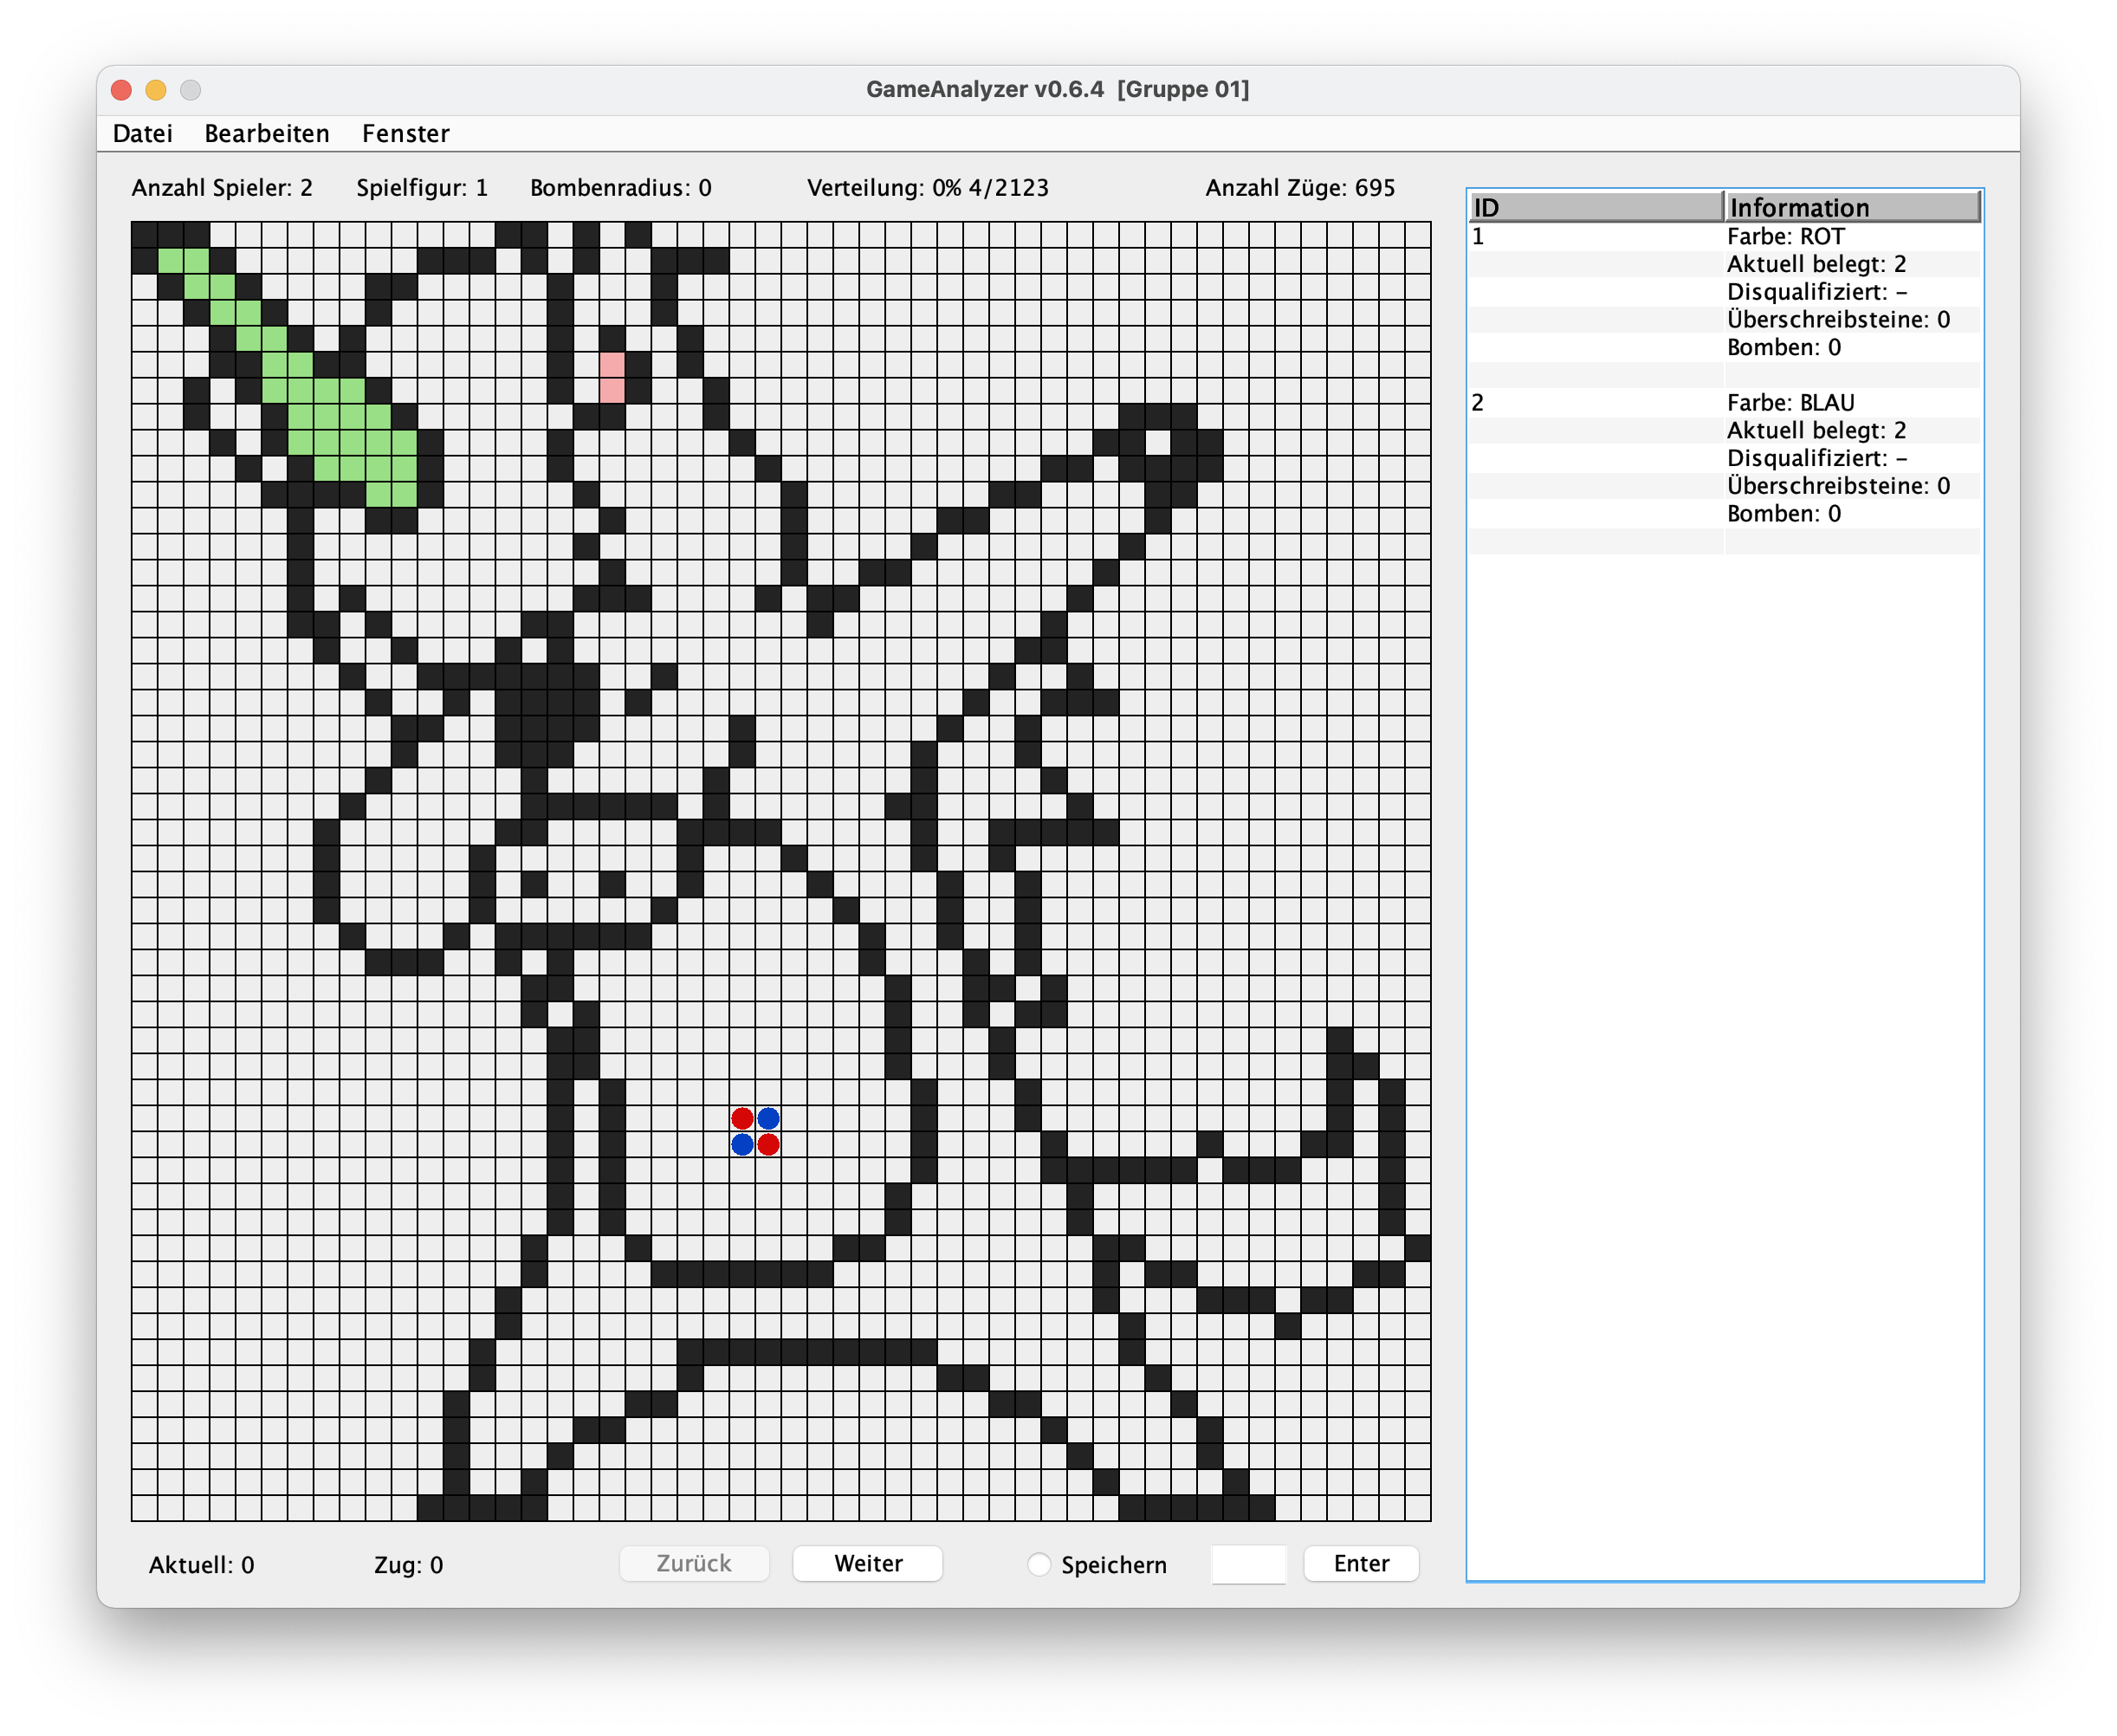
\includegraphics[width=0.8\linewidth]{pics/startscreen}
    \captionof{figure}[Startbildschirm GameAnalyze]{Startbildschirm GameAnalyze nach Auswahl einer Logdatei.}
    \label{fig:gameanalyze-start}
\end{minipage}
\vspace{1em}

Mit den Tasten Weiter und Zur\"uck kann man das Spiel in beide Richtungen durchlaufen.
In der rechten Tabelle werden alle Spieler angezeigt.
Zudem kann man darin nachschauen wie viele \"Uberschreibsteine, Bomben bzw.\ Spielsteine sie jeweils aktuell haben.
Ebenfalls ist zu sehen, welche Farbe sie haben und gegebenenfalls wann sie disqualifiziert werden.
Man erh\"alt weiterhin Informationen dar\"uber, wie viele Spielz\"uge es gibt und wie viel Prozent an Spielsteinen aktuell belegt sind.
Zudem kann unter Datei $\rightarrow$ Exportieren der aktuelle Stand der Karte exportiert werden, damit der Client die Karte mit dem gew\"unschten Spielstand wieder einlesen kann.
Falls Transitionen existieren, k\"onnen diese unter Bearbeiten ein- bzw.\ ausgeschaltet werden.

\subsection{Erreichbarer Felder anzeigen}\label{subsec:erreichbarer-felder-anzeigen}
Damit keine Spielfelder betrachtet werden m\"ussen die auf dieser Karte garnicht erreichbar sind, entwickelt unser Team einen MapAnalyzer, der zu Beginn des Spieles unerreichbare Positionen aus der Karte herausrechnet.
Welche Felder erreichbar bzw.\ nicht erreichbar sind kann man sich im GameAnalyzer ebenfalls anzeigen lassen.
Dazu geht man auf Fenster $\rightarrow$ Erreichbare Spielfelder.
Nun wird ein Fenster ge\"offnet, wie in Abbildung~\ref{fig:reachable-fields} zu sehen ist.

\vspace{1em}
\begin{minipage}{\linewidth}
    \centering
    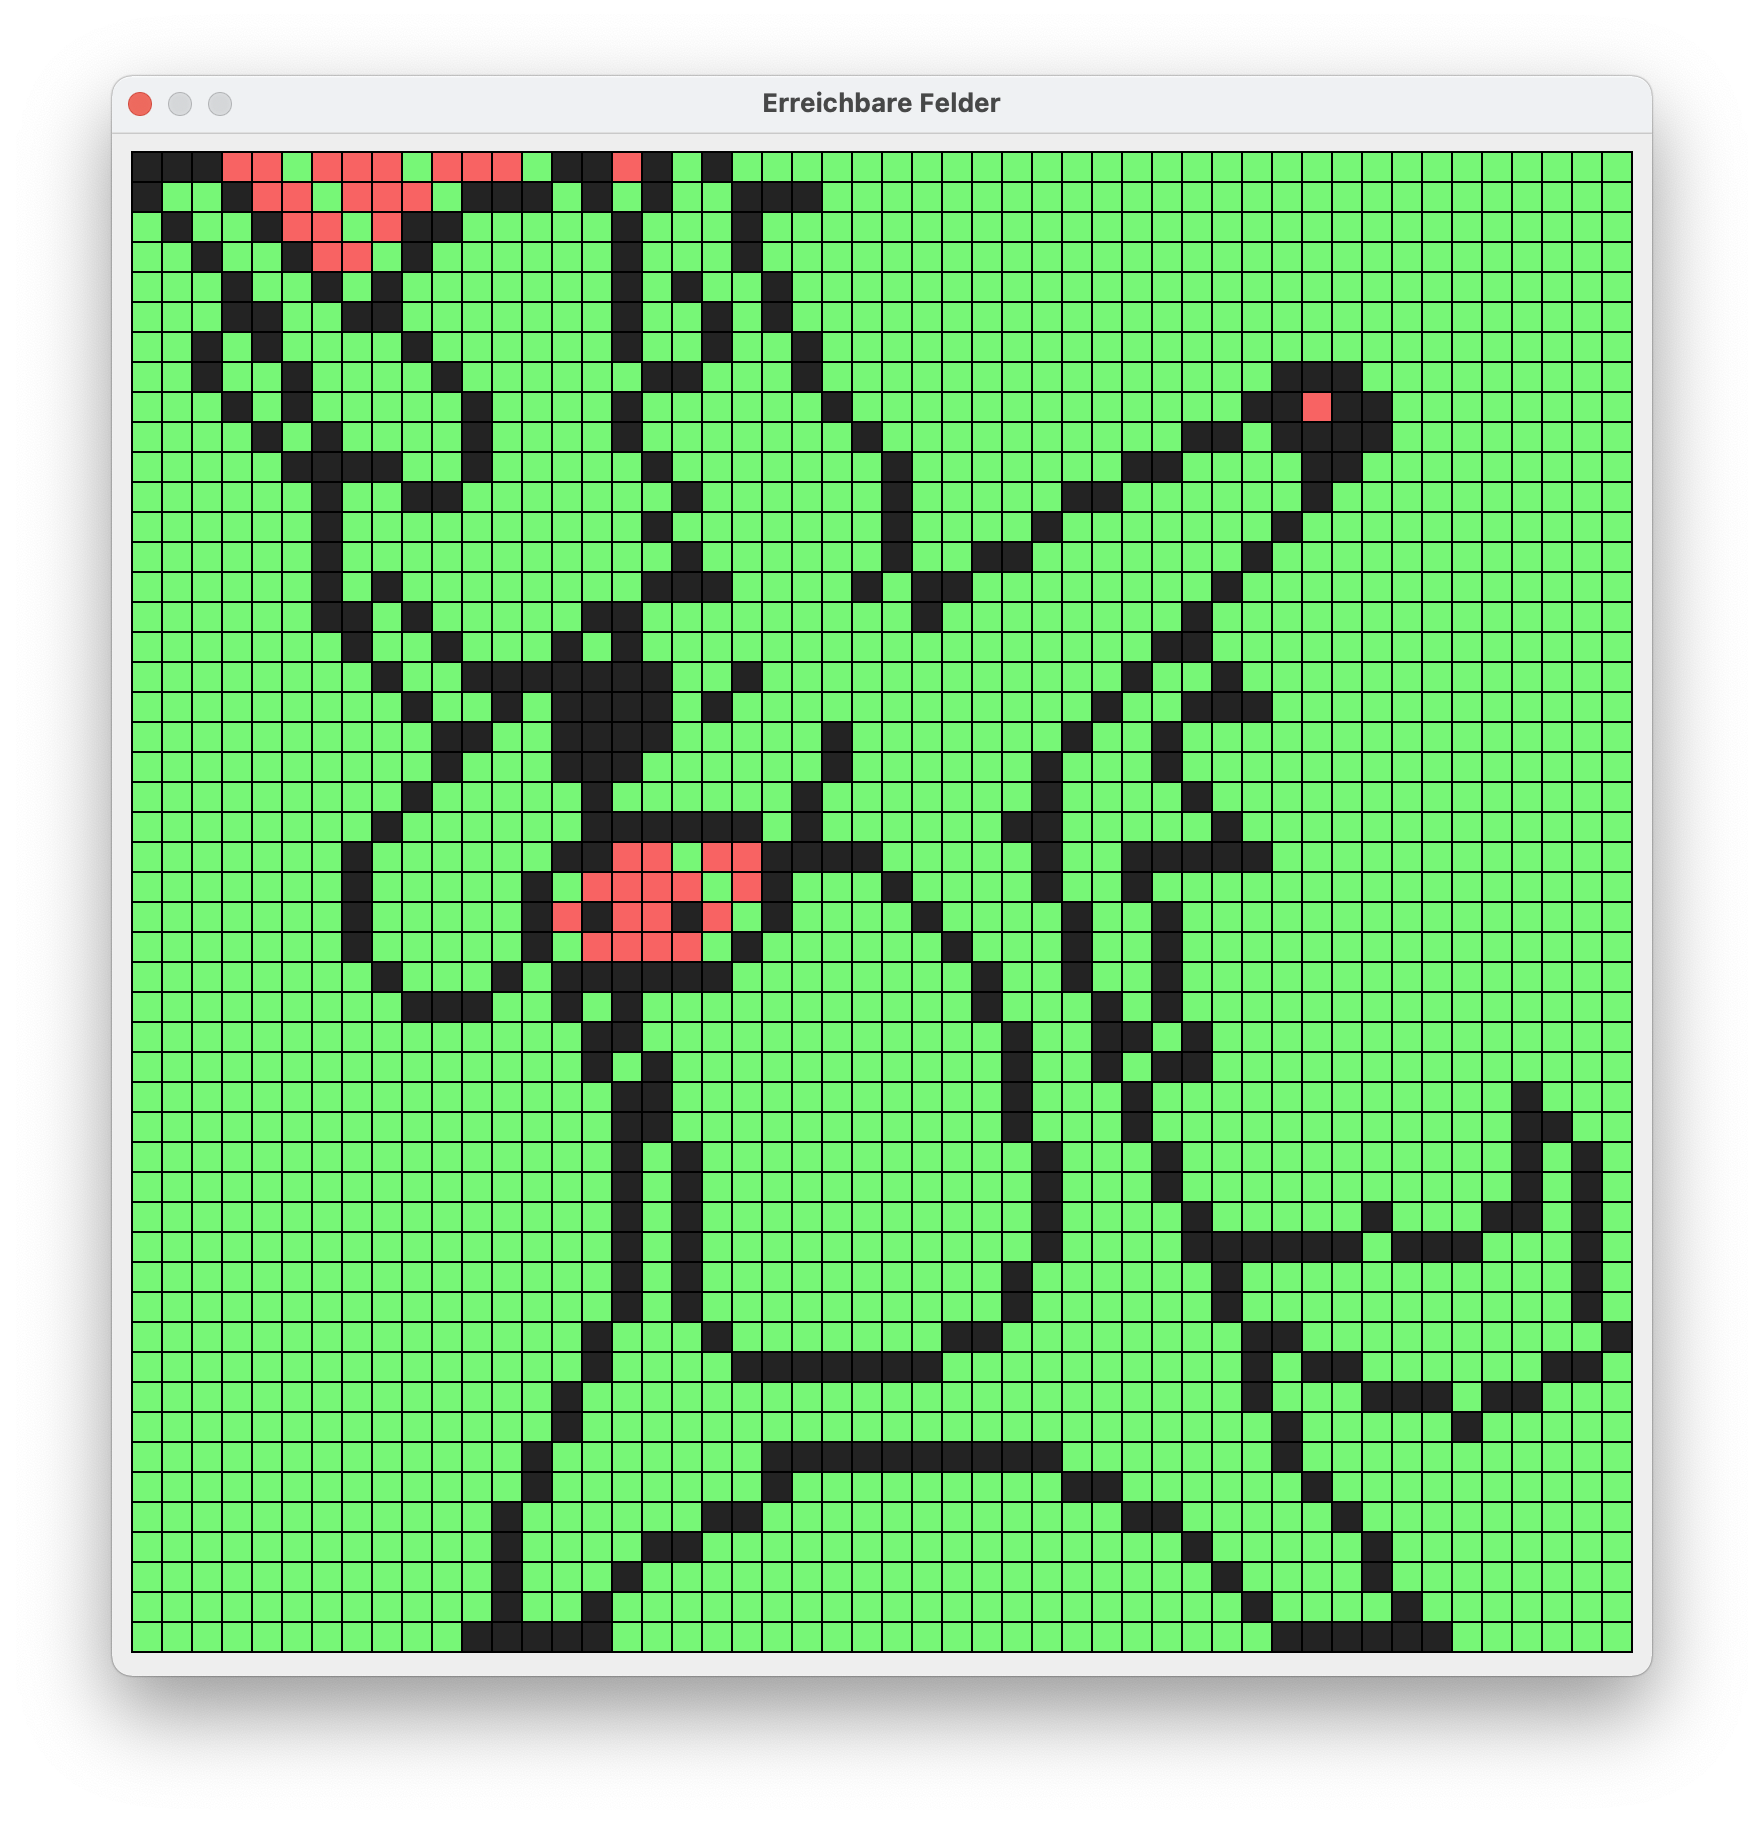
\includegraphics[width=0.6\linewidth]{pics/reachable-fields}
    \captionof{figure}[Anzeige unerreichbarer Felder]{Fenster um unerreichbare Felder anzuzeigen.}
    \label{fig:reachable-fields}
\end{minipage}

Schwarze Felder bedeuten, dass es sich hier um ein Loch handelt und dieses Feld somit generell nicht zu erreichen sind.
Gr\"un erscheinen die Felder, die w\"ahrend des Spieles erreichbar sind (Was jedoch nicht bedeutet, dass alle erreicht werden m\"ussen).
Rote Felder symbolisieren unerreichbare Felder w\"ahrend des gesamten Spieles.
(Mehr Informationen siehe Kapitel~\ref{sec:erreichbare-spielfelder})

\subsection{Detaillierter Statistiken anzeigen}\label{subsec:detaillierter-statistiken-anzeigen}
Unter dem Reiter Fenster kann man sich die unterschiedlichen Statistiken anzeigen lassen.
Wie Sie in Abbildung~\ref{fig:heuristic} sehen k\"onnen, wird damit der gesamte Zustand eines Spielers w\"ahrend des Spieles angezeigt.
Dabei wird immer die aktuelle Implementierung verwendet.

\vspace{1em}
\begin{minipage}{\linewidth}
    \centering
    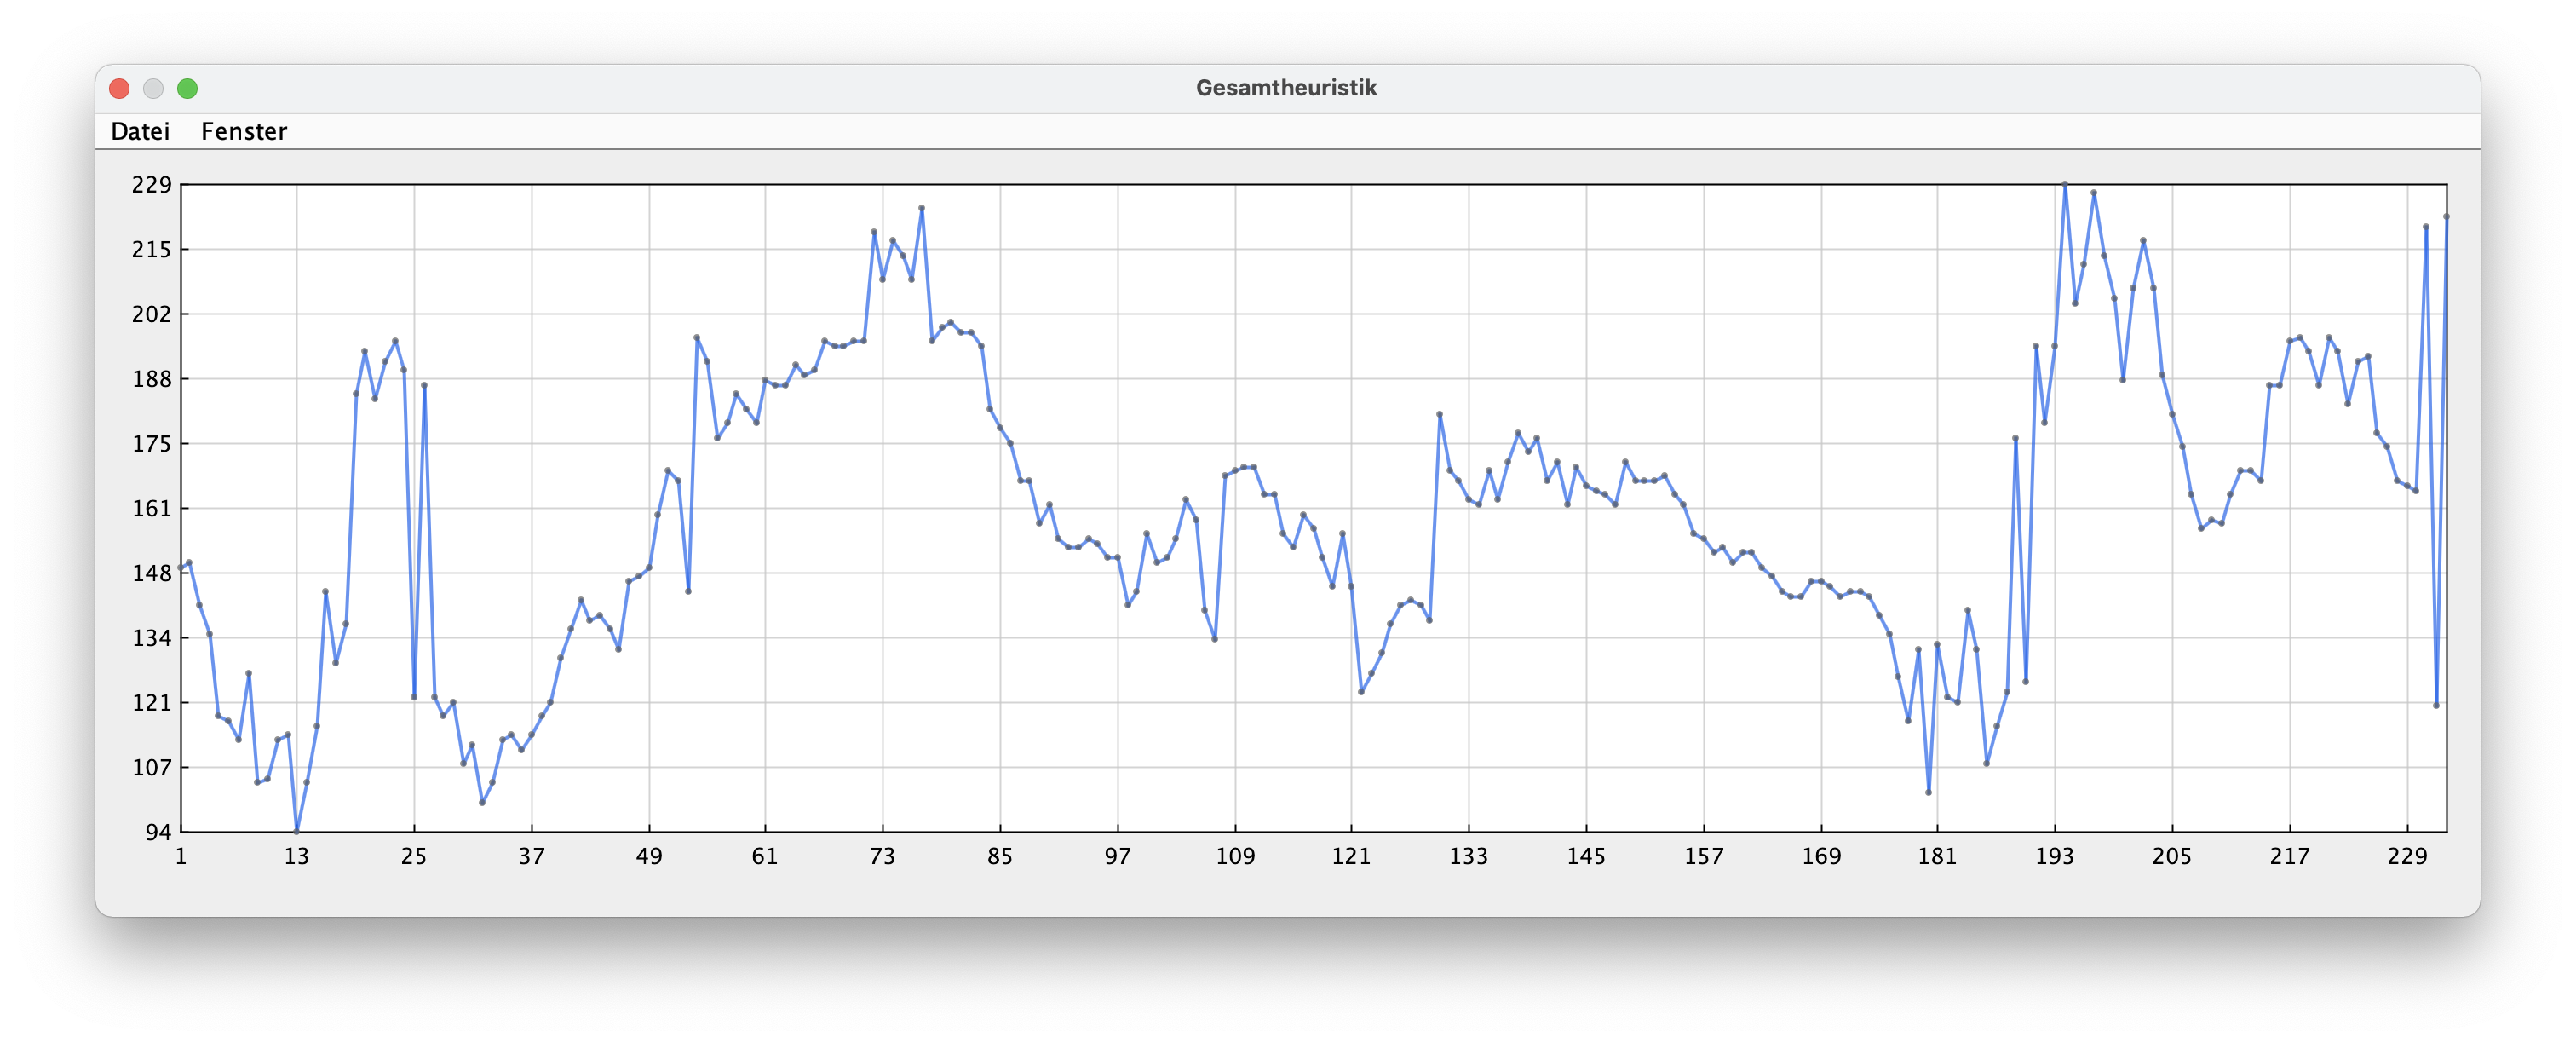
\includegraphics[width=0.8\linewidth]{pics/heuristic}
    \captionof{figure}[Grafik der Heuristik]{Fenster um aktuelle Heuristik anzuzeigen.}
    \label{fig:heuristic}
\end{minipage}
\vspace{1em}

M\"ochte man Zust\"ande der Heuristik f\"ur sp\"ater speichern, kann man sich diese selbstverst\"andlich exportieren lassen und mit Grafiken in der Zukunft vergleichen.
Ein solcher Vergleich kann nat\"urlich auch dazu genutzt werden, um unterschiedliche Spieler bzw.\ Varianten miteinander in Relation zu setzen.
Dies haben Sie bereits in Kapitel~\ref{subsubsec:vergleich-der-algorithmen} gesehen.

\subsection{Nutzen der Spielanalyse}\label{subsec:nutzen-der-spielanalyse}
Die Entwicklung der Spielanalyse ist ein zeitintensiver Prozess.
Es werden des \"Ofteren Spiele gegen andere Teams \"uber die Plattform Matchpoint gespielt.
Im Anschluss werden die Logdateien an die Gruppen verteilt, damit man eventuelle Abst\"urze finden oder auch generell den Spielverlauf anzeigen und verbessern kann.
Ein solches Turnier liefert oft mehrere Hunderte Logfiles, die man sich am Besten alle genaustens anschauen sollte.
Diese Software tr\"agt wesentlich dazu bei, dass dies f\"ur die Beteiligten in \"uberschaubarer Zeit und noch dazu sehr detailliert m\"oglich ist.
Es ist ebenfalls m\"oglich eine Karte einzulesen, damit man nicht extra ein Spiel mit zugeh\"origer Logdatei erh\"alt.
Man kann auch unter Bearbeiten $\rightarrow$ Manuelle Spielf\"uhrung h\"andisch das Spiel so kontrollieren wie man m\"ochte.
Zudem bietet dieses Fenster die M\"oglichkeit das manuell bearbeitete Spiel zu exportieren, um anschlie"send vom Server gelesen zu werden.


\bigskip
\newpage